\section{Motivation for Lightweight Imbalance Techniques} \label{sec:motivation}
% Imbalanced class distributions pose a persistent challenge in machine learning, especially for multi-class classification. A wealth of sophisticated methods have been proposed to improve learning from imbalanced data \cite{Chen2024,Ghosh2024}.
% %These include data-level techniques (\textit{e.g. complex oversampling and undersampling schemes}), algorithm-level strategies (\textit{cost-sensitive learning that adjusts class weight in the loss function}), advanced ensemble methods (\textit{bagging/boosting ensembles tailored to imbalance}), and specialized deep long-tail recognition networks \cite{Chen2024}. 
% While such state-of-the-art approaches can boost minority-class accuracy, they typically do so at the expense of high computational cost and added complexity. For example, boosting-based ensemble solutions must train many weak learners in sequence; this iterative process significantly increases training time and resource requirements, especially on large datasets. Chen et al. \cite{Chen2024} observe that although ensembles improve performance, a notable drawback of methods like AdaBoost is the “relatively higher computational cost” due to multiple training iterations and updates, which can render them impractical for large-scale tasks. 

% Similarly, deep cost-sensitive models require careful tuning of class weight hyperparameters or modified loss functions, and achieving the right balance can be complex. Long-tailed recognition networks (\textit{designed for extreme class imbalance}) often introduce additional network branches or expert subnetworks to better learn tail classes. 
% %A prominent example is the Bilateral-Branch Network (BBN) , which trains separate feature extractor and classifier branches for head and tail classes \cite{Ghosh2024}. Such architectures improve recognition of rare classes but substantially increase model size and training complexity. Likewise, generative oversampling methods train auxiliary generative models (\textit{e.g. GAN-based synthetic data generation}) to augment minority classes. 
% Although effective in certain cases, these generative approaches add considerable overhead. Ghosh et al. \cite{Ghosh2024} highlight that many GAN-based oversampling techniques suffer from slow training due to the extra computations (\textit{for instance, computing nearest neighbors in each mini-batch to generate new samples}), which can significantly slow down learning on large-scale problems. 
%In summary, the latest surveys \cite{Chen2024,Ghosh2024} concur that many cutting-edge imbalance solutions—ensemble frameworks, deep cost-sensitive algorithms, long-tail networks, and generative data augmenters—tend to be resource-intensive, with complex designs that may yield diminishing returns relative to their computational expense. Indeed, Chen et al. \cite{Chen2024} note that such methods often exhibit “high computational complexity, complex model design, and no guaranteed substantial improvements”, underscoring the need for more efficient alternatives. 


While a wealth of sophisticated methods have been proposed to improve learning from imbalanced data, state-of-the-art approaches often boost minority-class accuracy at the expense of high computational cost and added complexity. For example, boosting-based ensembles must train many weak learners in sequence, a process that significantly increases training time and resource requirements. Chen et al. \cite{Chen2024} note that this \textit{relatively higher computational cost} can render such methods impractical for large-scale tasks.

\begin{figure*}[t]
\centering
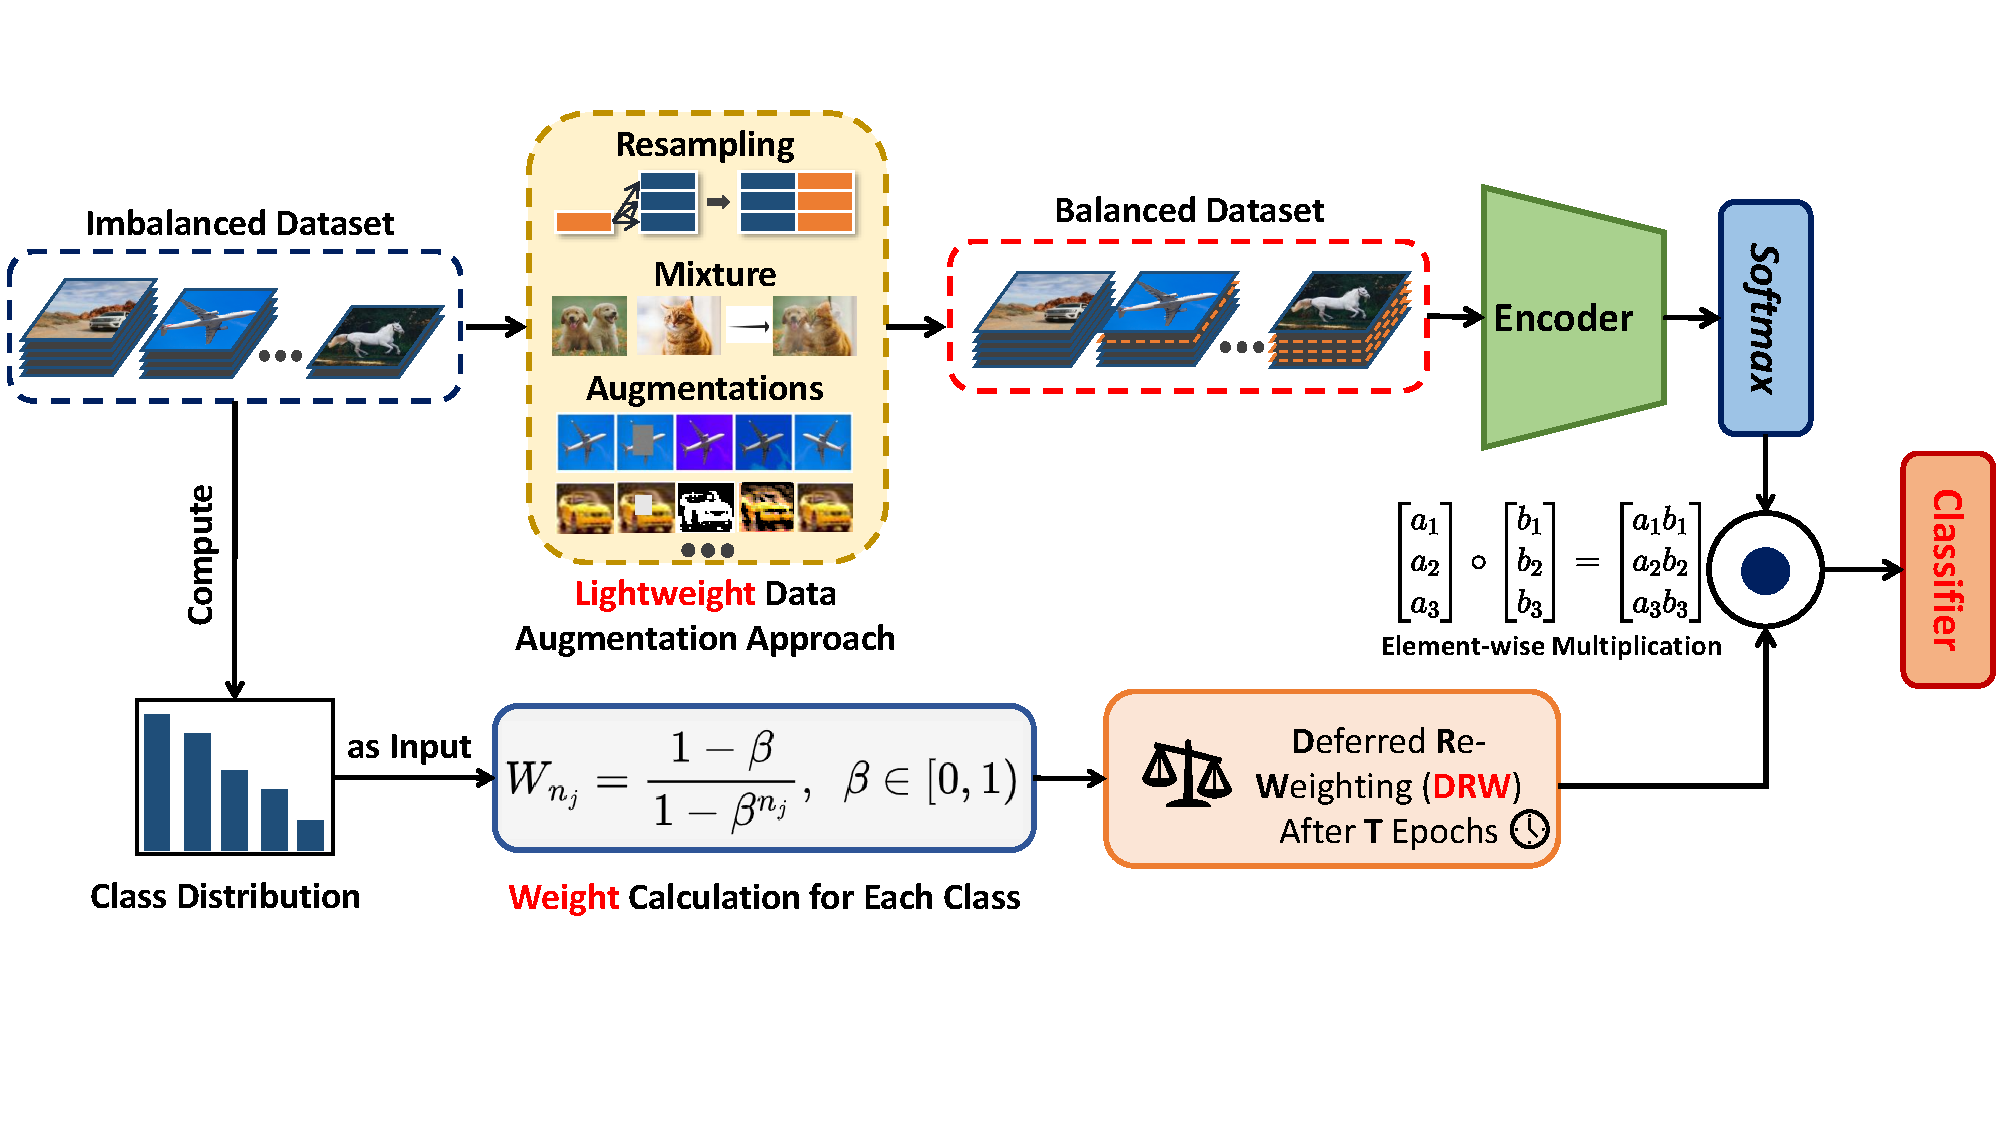
\includegraphics[width=\textwidth, clip, trim=0cm 2.5cm 0cm 1.5cm]
{Imbalanced-final}
    \caption{An overview of lightweight data augmentation techniques for imbalance learning.}
    \label{fig:imbalance_learning}
\end{figure*}

Similarly, other strategies incur significant overhead due to complex designs or auxiliary modules. Generative approaches like DeepSMOTE~\cite{dablain2022deepsmote}, which uses an encoder-decoder to synthesize minority samples, can lead to a computational overhead of 1.5 to 2 times the baseline cost. Ghosh et al. \cite{Ghosh2024} highlight that many GAN-based techniques suffer from slow training due to extra computations, such as finding nearest neighbors to generate new samples. Other methods, like MAMix~\cite{cheng2023smote}, introduce adaptive controllers that can increase training time by 15–25\%. In contrast, some techniques demonstrate that performance gains are possible without a heavy price; for instance, LDAM-DRW~\cite{cao2019learning} modifies a deferred class weighting schedule and adds negligible cost relative to standard training.
% \ha{consider putting a clock to signify a delay}

These concerns motivate the adoption of lightweight techniques for class imbalance, which aim to rebalance learning at much lower computational cost. Rather than fundamentally altering the model architecture or training an army of classifiers, lightweight methods adjust the data seen by a standard model in simple but effective ways~\cite{lightweight-longtailed, lightweightfightingmodel}. Two widely practiced families of such techniques are data augmentation and sample weighting/sampling strategies. Data augmentation inflates the effective training set by applying label-preserving transformations to input examples, thereby improving generalization for minority classes without collecting new data. Notably, modern augmentation policies like AutoAugment \cite{cubuk2018autoaugment} and RandAugment \cite{cubuk2019randaugment} can be plugged into training pipelines to automatically generate diverse image variants. 
%(\textit{through random crops, flips, color jittering, rotations, etc.}) with virtually no additional model overhead. These methods require only minor computational effort for image transformations, yet can substantially enrich the variability of rare class samples. Likewise, simple augmentation tricks such as Cutout \cite{devries2017cutout} help the model learn more robust features for all classes, including the minority ones, without any increase in model parameters. Because augmentation operations are performed on-the-fly on the CPU/ GPU during data loading, they are highly efficient and scalable. In imbalanced settings, augmentation can be particularly beneficial when applied more aggressively to minority class examples, effectively boosting their presence. For instance, recent studies have explored the enhancement of majority class samples and transferring them to enrich minority classes, as well as learning augmentation policies tailored to long-tailed distributions (\textit{to avoid simply magnifying the imbalance}) \cite{Chen2024}. 
Overall, data augmentation offers a lightweight, domain-agnostic tool to improve class balance: one can obtain significant gains in minority-class recognition by simply leveraging existing images more effectively, rather than training complex new models. 

Another efficient remedy to imbalance is to adjust the sampling or weighting of training examples, so that minority classes are seen more frequently by the learner. Many deep learning pipelines support weighted random sampling, wherein each data instance is sampled with probability inversely proportional to its class frequency. This yields mini-batches that are approximately class-balanced on average, without altering the model itself. Implementing such a scheme is straightforward and incurs negligible overhead beyond the bookkeeping of sample weight. 
% \ha{shall we do font change to WeightedRandomBatchSample, WeightedFixedBatchSample and the like} 
A related technique is to use a fixed sampling ratio per class and tune a parameter $\alpha$ that controls how strongly the sampling favors minority classes. A small $\alpha$ might slightly up-sample rare classes, whereas a larger $\alpha$ moves closer to fully balanced sampling. By varying $\alpha$, one can smoothly trade off between biasing towards the minority class vs. preserving the original data distribution. Importantly, these sampling strategies are easy to integrate into training loops and avoid the need for any additional model training. They essentially reallocate existing data resources in a smarter way. Crucially, such data rebalancing can be combined with data augmentation for compound effect: e.g., one might oversample the rare classes and apply stronger augmentation to them, yielding a diverse set of synthetic minority examples at very low cost. Unlike generate new samples or fine-tuning a complicated cost-sensitive loss schedule, sampling and augmentation methods keep the training pipeline simple and computationally cheap. 

While both Mixup and Deferred Re-Weighting (DRW) have been extensively studied, our proposed Imbalanced Lightweight Hybrid (ILWH) introduces a distinct integration of these two paradigms within a unified, resource-efficient framework. Below, we outline the conceptual and practical distinctions between ILWH and related approaches such as MAMix, DeepSMOTE, and LDAM-DRW.

% Existing imbalance-handling strategies often incur significant additional computation due to complex model designs or auxiliary optimization modules. 
% DeepSMOTE~\cite{dablain2022deepsmote}, for example, employs an encoder--decoder generator to synthesize minority samples in latent space, leading to a computational overhead of approximately $1.5\times$ to $2\times$ the baseline cost. 
% MAMix~\cite{cheng2023smote} introduces an adaptive margin controller that dynamically adjusts interpolation ratios, resulting in a reported $15$--$25\%$ increase in training time. 
% In contrast, LDAM-DRW~\cite{cao2019learning} modifies only the deferred class weighting schedule and therefore adds negligible cost ($<5\%$) relative to standard Empirical Risk Minimization (ERM).
% Beyond their elegance and ease of implementation, lightweight imbalance techniques have demonstrated competitive performance in practice. On standard vision benchmarks with many classes — such as CIFAR-10, CIFAR-100, and SVHN — simple oversampling or class-balanced sampling strategies, together with appropriate augmentations, often close much of the accuracy gap between minority and majority classes. For example, on long-tailed versions of CIFAR, balancing the mini-batches by oversampling the scarce classes can markedly improve minority-class recall, sometimes rivaling the results of far more elaborate algorithms. Likewise, applying AutoAugment or RandAugment policies has been shown to boost overall accuracy on imbalanced CIFAR-100 with minimal tuning, nearly matching specialized long-tail methods in some studies. Indeed, an influential work by Kang et al. (2019) found that a relatively simple two-phase training (first learning a feature backbone on the natural imbalanced data, then re-training the classifier with class-balanced sampling) achieved state-of-the-art results on long-tailed recognition benchmarks, highlighting that complex imbalanced-learning machinery is not always necessary. This insight, echoed by Ghosh et al. \cite{Ghosh2024}, reinforces the appeal of lightweight solutions: they can yield robust models that perform well across all classes without the burden of extensive additional computation. In scenarios where computing resources are limited — e.g. deploying models on mobile, edge, or embedded devices — such efficient techniques are particularly attractive. A mobile or IoT device may not accommodate large ensemble models or GAN generators, but can readily handle a bit of extra data augmentation or a modified sampling scheme during training. By adopting these resource-friendly methods, one can mitigate class imbalance while keeping the model lean and the training requirements modest.

In summary, the high cost and complexity of many modern imbalance-learning algorithms motivate a turn towards lightweight alternatives that are easier to deploy and scale. 
%Data augmentation and smart sampling are two pillars of this approach, offering significant practical benefits: they are simple to implement, impose minimal computational overhead, and yet substantially improve model fairness and accuracy across classes. 
%Equally important, they integrate seamlessly into existing training pipelines on common datasets (\textit{such as CIFAR-10, CIFAR-100, CINIC-10, SVHN-10, TinyImageNet-200}) and do not require specialized architectures or costly procedures. This makes them ideal for researchers and practitioners aiming to address class imbalance under real-world constraints. 
The evidence so far suggests that these lightweight methods can performance competitiveness with far more complex techniques \cite{Chen2024,Ghosh2024}, striking an excellent balance between effectiveness and scalability. Therefore, it is highly compelling to leverage such approaches for imbalanced multi-class classification problems, particularly when working in resource-constrained environments or seeking broadly applicable, easy-to-tune solutions. We build on this motivation and advocate for imbalance mitigation strategies that remain accessible and computationally light-weight, without sacrificing too much in terms of accuracy.
